\documentclass[draft=True]{revtex4-2}
\newcommand{\zreco}{\ensuremath{\cos{(\theta_z^{reco})}}}
\newcommand{\ztrue}{\ensuremath{\cos{(\theta_z^{true})}}}
\newcommand{\emm}{\ensuremath{\epsilon_{\mu\mu}}}
\newcommand{\emt}{\ensuremath{\epsilon_{\mu\tau}}}
\newcommand{\ett}{\ensuremath{\epsilon_{\tau\tau}}}
\newcommand{\ep}{\ensuremath{\epsilon^\prime}}
\renewcommand{\ne}{\nu_e}
\newcommand{\nm}{\nu_\mu}
\newcommand{\nt}{\nu_\tau}
\newcommand{\ane}{\bar\nu_e}
\newcommand{\anm}{\bar\nu_\mu}
\newcommand{\ant}{\bar\nu_\tau}
\usepackage{physics,amsmath, amsfonts, siunitx, amssymb, graphicx}
\usepackage[utf8]{inputenc}
\usepackage{hyperref}
\begin{document}
\section{Methodology}
The neutrino flux at the detector is calculated by propagating the atmospheric neutrino flux~\cite{hondapaper} through the Earth by solving the 
Schrödinger equation for varying density. The Earth density profile is taken from the PREM~\cite{PREM}. 
The oscillation probability $P_{\alpha \beta}$ then acts as a weight, yielding the propagated flux at detector level for flavor $\beta$ as 
\begin{align}\label{eq:propFlux}
    \phi_\beta^\text{det} = \sum_\alpha \frac{\dd^2 \phi_\alpha^\text{atm}}{\dd E^t \dd \cos{\theta^t_z}} P_{\alpha\beta}\,,
\end{align}
where we sum over the initial lepton flavors $\alpha \in \{e,\mu, \bar{e}, \bar{\mu}\}$.
\subsection{IceCube}\label{ch:ICmethod}
The event rate for each bin reads
\begin{align}\label{eq:ICevents}
    N_{ij} &= T \int_{(\cos{\theta_z^r})_i}^{(\cos{\theta_z^r})_{i+1}} \dd \cos{\theta^r_z} \int_{E^r_{j}}^{E^r_{j+1}} \dd E^r \int_0^\pi R(\theta^r,\theta^t) \dd \cos{\theta^t} \int_0^\infty R(E^r,E^t) \dd E^t
    \times \left[ \sum_\beta \phi_\beta^\text{det}  A^\text{eff}_\beta\right]\,,
\end{align}
where $T$ is the live time of the detector, and $A^\text{eff}_\beta$ its effective area for flavor $\beta$. We use the effective area of the 86 string configuration made public by the IceCube collaboration~\cite{ICaeff}. $R(x^r,x^t)$ is a Gaussian resolution function, 
which is responsible for the smearing between the reconstructed and true parameters $x^r$ and $x^t$, respectively. It takes the form 
\begin{align}
    R(x^r, x^t) = \frac{1}{\sqrt{2\pi} \sigma_{x^r}} \exp\left[\frac{(x^r-\mu(x^t))^2}{2\sigma_{x^r}^2}\right]\,.
\end{align}
Assuming no bias in the reconstruction, the mean of the Gaussian can be taken as $\mu(x^t) = x^t$. As seen in Fig.~\ref{fig:IC_MC_counts}, the distribution of 
simulated events is skewed. Instead, we assume a log-normal distribution between $E^{true}$ and $E^{reco}$, and train a Gaussian Process Regressor on the dataset~\cite{IC2016}, from which
we can extract a predicted mean and standard deviation for each $E^{reco}$. We then sample values from this distribution to yield 
the points of $E^{true}$ at which to integrate over. 

In Icecube, the zenith angle resolution for track-like events is less than $\SI{2}{\degree}$, making $\ztrue$ coincide with $\zreco$ for our study~\cite{IC2020}.
\begin{figure}[!tb]
    \begin{center}
       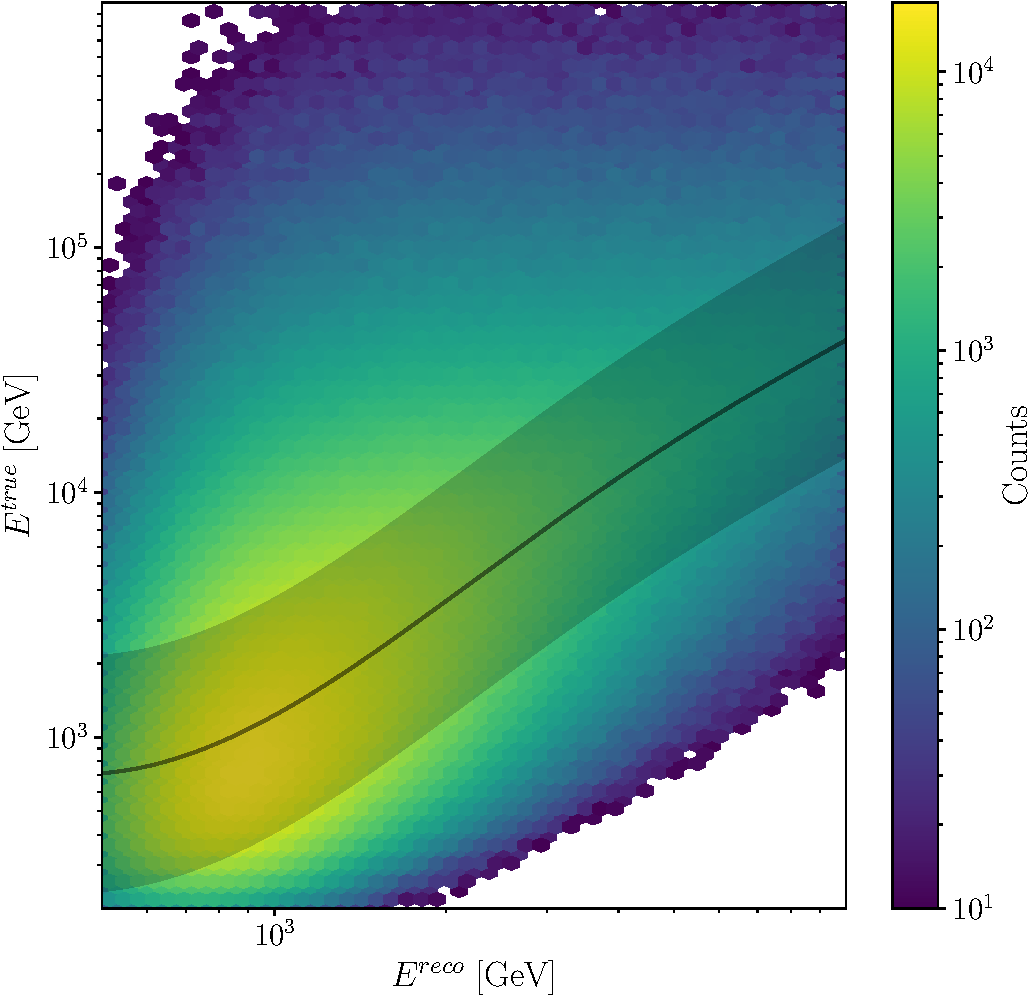
\includegraphics[width=0.4\linewidth]{figures/IC_MC_gpr.pdf}
    \end{center}
    \caption{Relationship between the true and reconstructed muon energy in the IceCube MC sample~\cite{IC2016}}\label{fig:IC_MC_counts}. Shaded area shows the $99.9$th percentile limits predicted by the regressor trained on this set.
 \end{figure}
The data is from the IC86 sterile analysis~\cite{IC2020}.

\subsection{DeepCore}\label{ch:DCmethod}
In this part, we use the publically available DeepCore data sample~\cite{DC2019data} which is an updated version of what was used by the 
IceCube collaboration in an $\nu_\mu$ disapprearance analysis~\cite{DC2018mudisappearance}.

The detector systematics include ice absorption and scattering, and overall, lateral, and head-on optical efficiencies of the DOMs. 
They are applied as correction factors using the best-fit points from the DeepCore 2019 $\nu_\tau$ appearance 
analysis~\cite{DC2019tauappearance}.

The data include 14901 track-live events and 26001 cascade-like events, both divided into eight 
$ \log_{10}E^{reco} \in [0.75,1.75]$ bins, and eight $\zreco \in [-1,1]$ bins.

The oscillation parameters are from the
best-fit in the global analysis in~\cite{nufit}: $\theta_{12} = \SI{33.44}{\degree},\, \theta_{13} = \SI{8.57}{\degree},\, \Delta m^2_{21} =  \SI{7.42}{\electronvolt^2}$, and we 
marginalize over $\Delta m^2_{31}$ and $\theta_{23}$.

Given a Monte Carlo simulation with weights $w_{k\beta}$, we can construct the event count as
\begin{align}\label{eq:MCevents}
    N_{ijk} &= C_{ijk}\sum_{\beta}w_{ijk,\beta} \phi_\beta^\text{det}\,,
\end{align}
where $C_{k\beta}$ is the correction factor from the detector systematic uncertainty and $\phi_\beta^\text{det}$ is defined as Eq.~\ref{eq:propFlux}. We have now substituted the effect of the Gaussian smearing 
by treating the reconstructed and true quantities as a migration matrix. 

\subsection{PINGU}\label{ch:PINGUmethod}
The methodology behind the PINGU simulations are the same as with our DeepCore study~\ref{ch:DCmethod}. We use the public MC~\cite{PINGUdata}, which allows us to construct the event count as in Eq.~\ref{eq:MCevents}.
However, since no detector systematics is yet modelled for PINGU, the correction factors $C_{ijk}$ are all unity.
As with the DeepCore data, the PINGU MC is divided into eight 
$\log_{10}E^{reco} \in [0.75,1.75]$ bins, and eight $\zreco \in [-1,1]$ bins for both track- and cascade-like events. 
We generate "data" by predicting the event rates at PINGU with the following best-fit parameters from~\cite{nufit}, except for the CP-violating phase which is set to zero for simplicity.

\begin{align}\label{eq:PINGUparams}
    &\Delta m^2_{21} =  \SI{7.42e-5}{\electronvolt^2},\hspace{0.5em} \Delta m^2_{31} =  \SI{2.517e-3}{\electronvolt^2}, \nonumber \\
    &\theta_{12} = \SI{33.44}{\degree},\hspace{1em} \theta_{13} = \SI{8.57}{\degree},\hspace{1em} \theta_{23} = \SI{49.2}{\degree}, \hspace{1em} \delta_\text{CP} = 0\,.
\end{align}



\section{Results}
For our analyses, we define our $\chi^2$ as
\begin{align} \label{eq:ICchisq}
    \chi^{2}(\hat{\theta},\alpha,\beta, \kappa)=\sum_{ijk} \frac{\left(N^\text{th}-N^\text{data}\right)_{ijk}^{2}}
    {\left(\sigma^\text{data}_{ijk}\right)^{2} + \left(\sigma^\text{syst}_{ijk}\right)^{2}}+ 
    \frac{(1-\alpha)^2}{\sigma_\alpha^2} + \frac{\beta^2}{\sigma_\beta^2}\,
\end{align}
where we minimize over the model parameters $\hat{\theta} \in \{\Delta m_{31}^2, \theta_{23}, \ep, \emt\}$, the penalty terms $\alpha$ and $\beta$, and the free parameter $\kappa$.
$N_{ijk}^\text{th}$ is the expected number of events from theory, and $N_{ijk}^\text{data}$ is the observed number of events in that bin. We set $\sigma_\alpha = 0.25$ as the atmospheric flux normalization error, and $\sigma_\beta = 0.04$ as the zenith angle slope error~\cite{hondapaper}. 
The observed event number has an associated Poissonian uncertainty $\sigma_{ijk}^\text{data} = \sqrt{N_{ijk}^\text{data}}$.

For IceCube, the event count takes the form
\begin{align}
    N^\text{th}_{ijk} = \alpha\left[1+\beta (0.5 + \zreco_i )\right] N_{ijk}(\hat{\theta})\,,
\end{align}
with $N_{ijk}(\hat{\theta})$ from Eq.~\ref{eq:ICevents} Here, we allow the event distribution to rotate around the median zenith of $-0.5$.

For DeepCore and PINGU, the event count takes the form
\begin{align}
    N^\text{th}_{ijk} = \alpha\left[1+\beta \zreco_i \right] N_{ijk}(\hat{\theta}) + \kappa N_{ijk}^{\mu_{atm}}\,,
\end{align}
with $N_{ijk}(\hat{\theta})$ from Eq.~\ref{eq:MCevents}. $N_{ijk}^{\mu_{atm}}$ is the muon background, which is left to float freely in the DeepCore analysis.
The background at PINGU can be considered neglible to first order~\cite{PINGUdata}, and we thus put $\kappa=0$ when calculating the PINGU $\chi^2$\,.
For IceCube, we set $\sigma_{ijk}^\text{syst} = f\sqrt{N_{ijk}^\text{data}}$.
For DeepCore, we use the provided systematic error distribution which accounts for both uncertanties in the finite MC statistics and in the data-driven 
muon background estimate~\cite{DC2019data}.




We plot the event pull $(N_{NSI} - N_{SI})/\sqrt{N_{SI}}$ where $N_{(N)SI}$ are the numbers of expected events
assuming (non-)standard interactions. This gives the normalized difference in the
number of expected events at the detector, and illustrates the expected sensitivity for the NSI parameters.

\begin{figure}[!tb]
    \begin{center}
       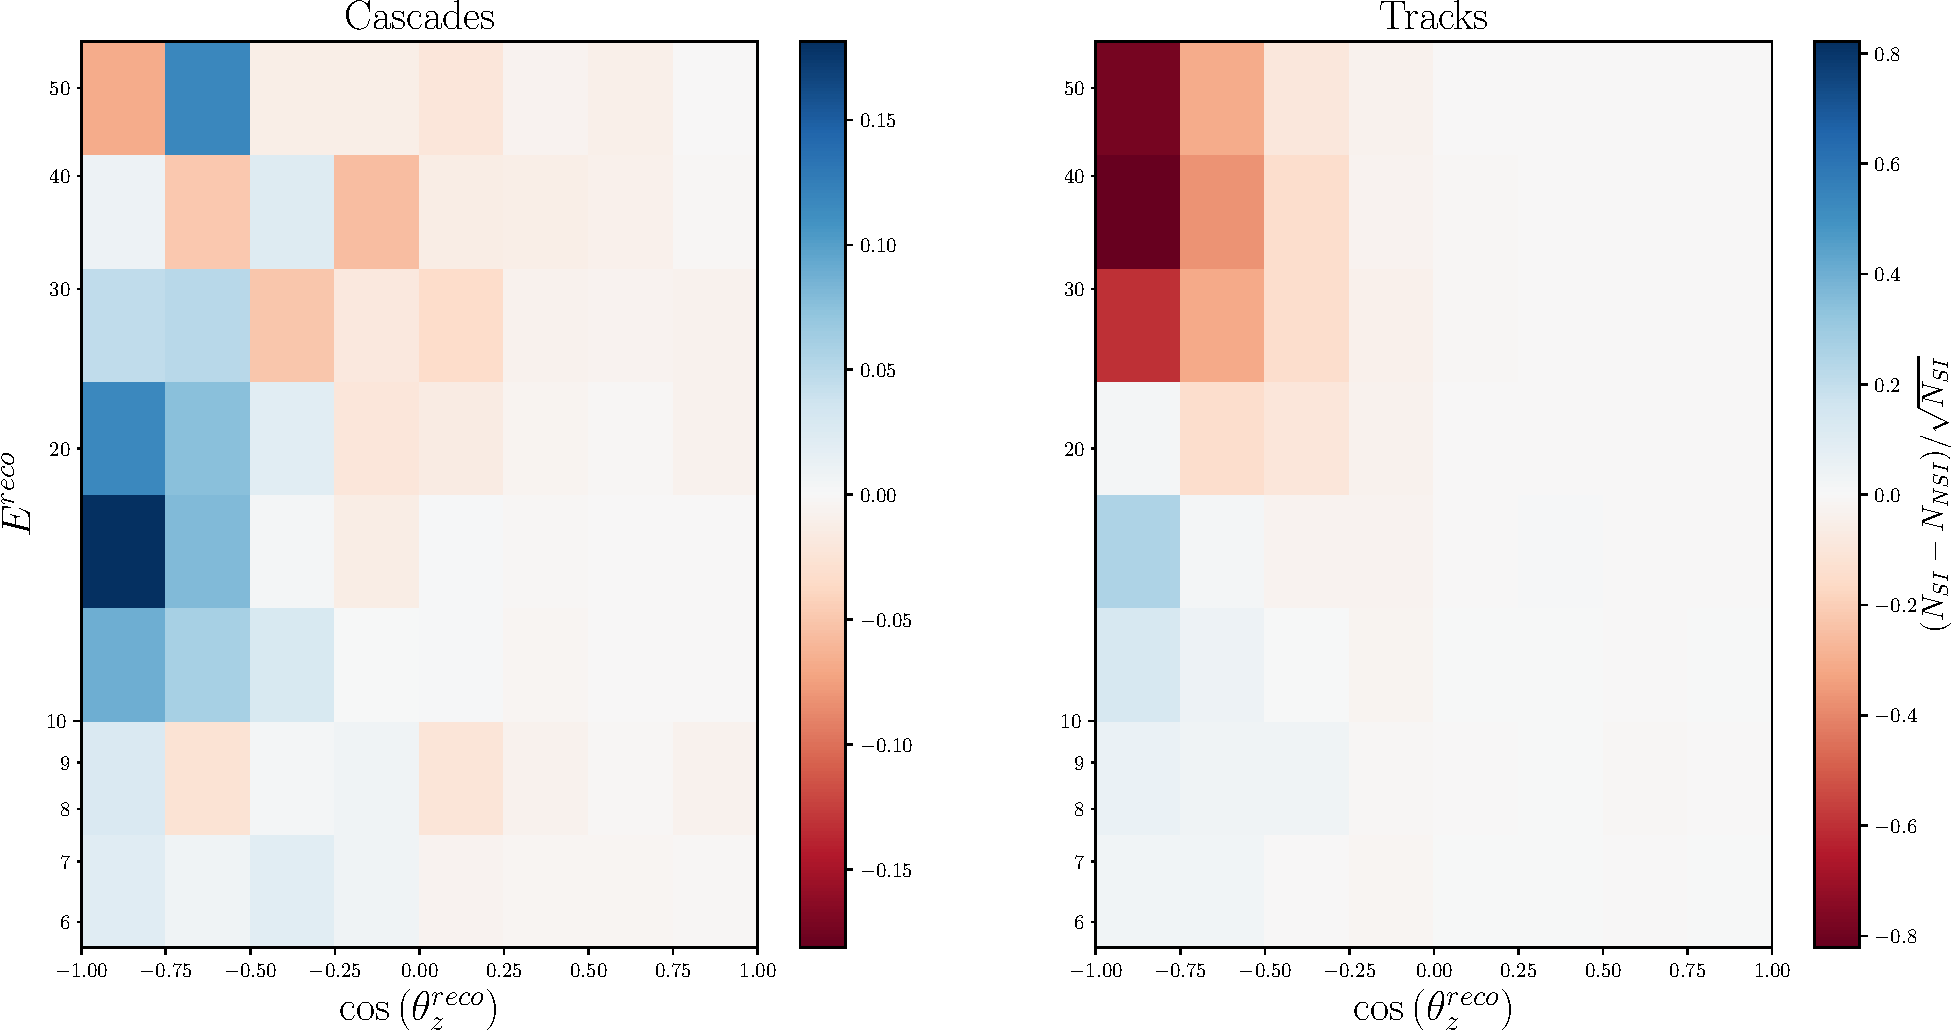
\includegraphics[width=0.7\linewidth]{figures/DC_event_pulls.pdf}
    \end{center}
    \caption{Expected pulls of predicted event numbers for DeepCore. We compare the NSI event count with $\emt=-0.05$
     to the standard interaction count}\label{fig:DC_event_pulls}
 \end{figure}

 \begin{figure}[!tb]
    \begin{center}
       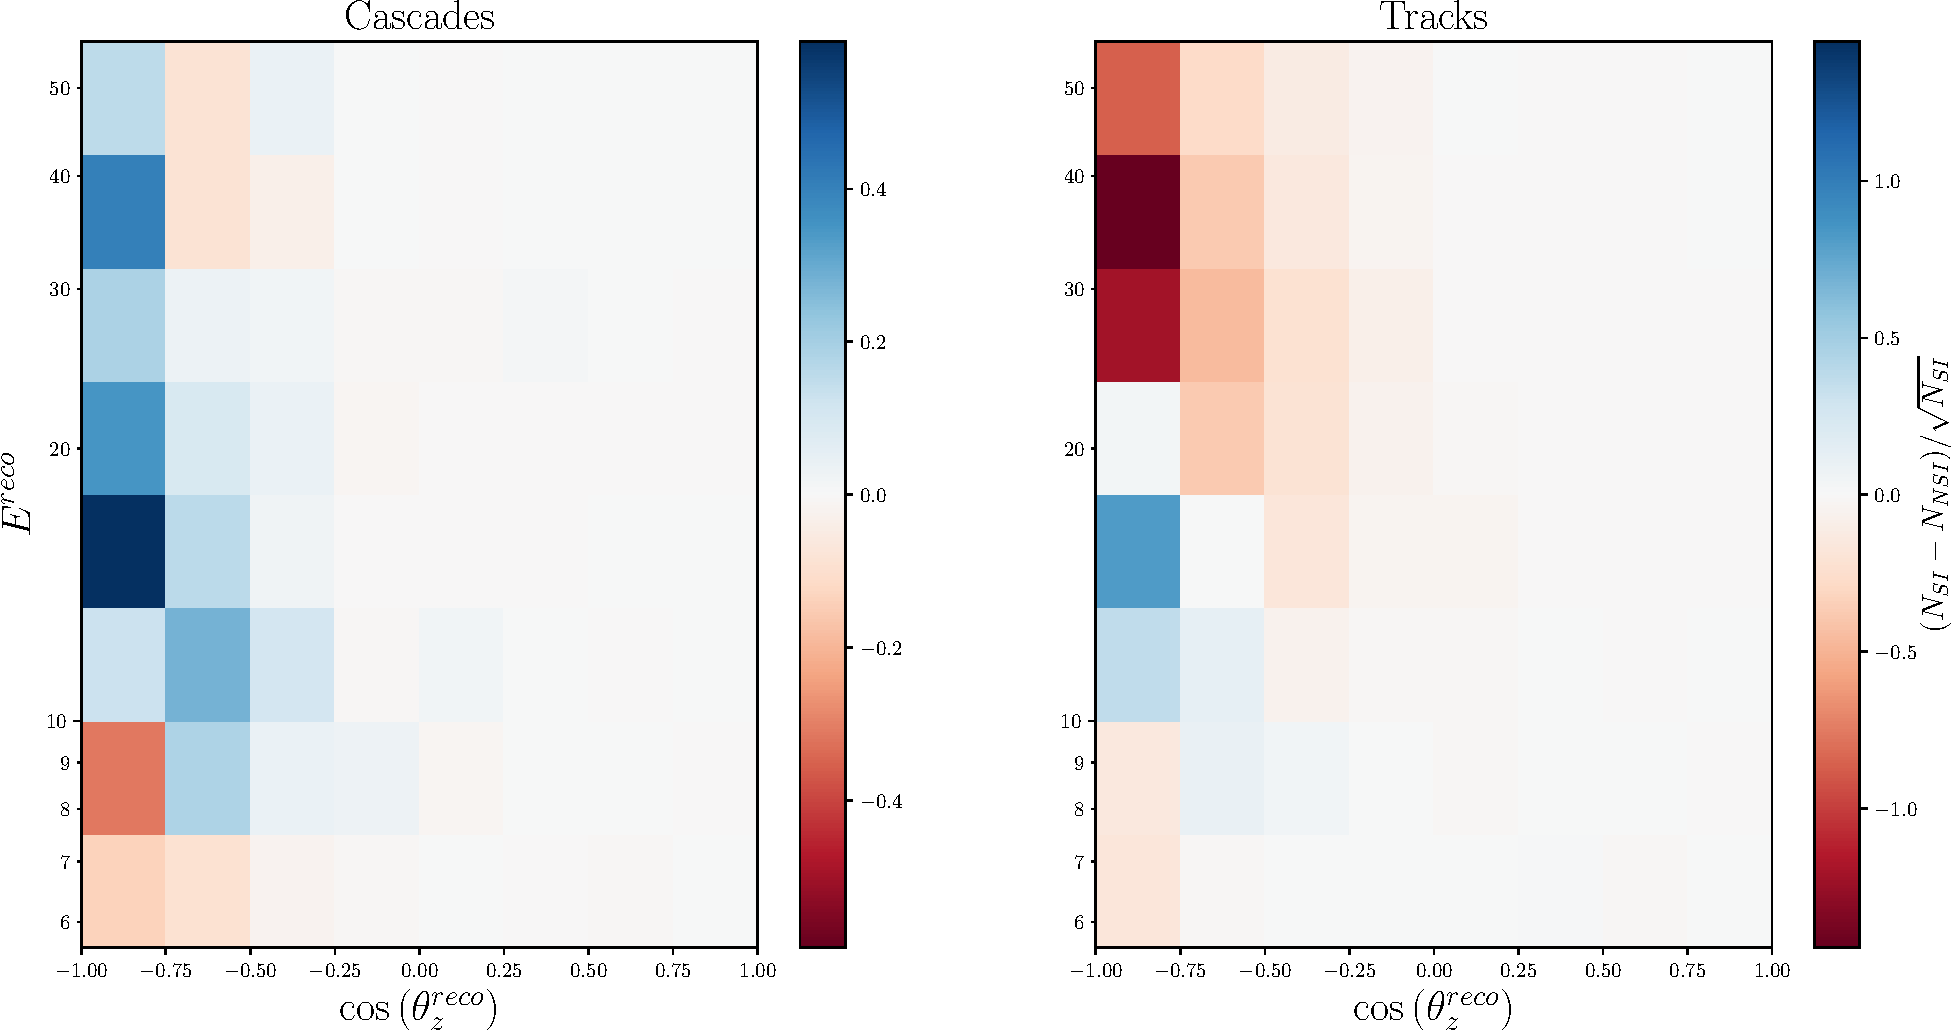
\includegraphics[width=0.7\linewidth]{figures/PINGU_event_pulls.pdf}
    \end{center}
    \caption{Expected pulls of predicted event numbers for PINGU. We compare the NSI event count with $\emt=-0.05$
    to the standard interaction count}\label{fig:PINGU_event_pulls}
 \end{figure}

 \begin{figure}[!tb]
    \begin{center}
       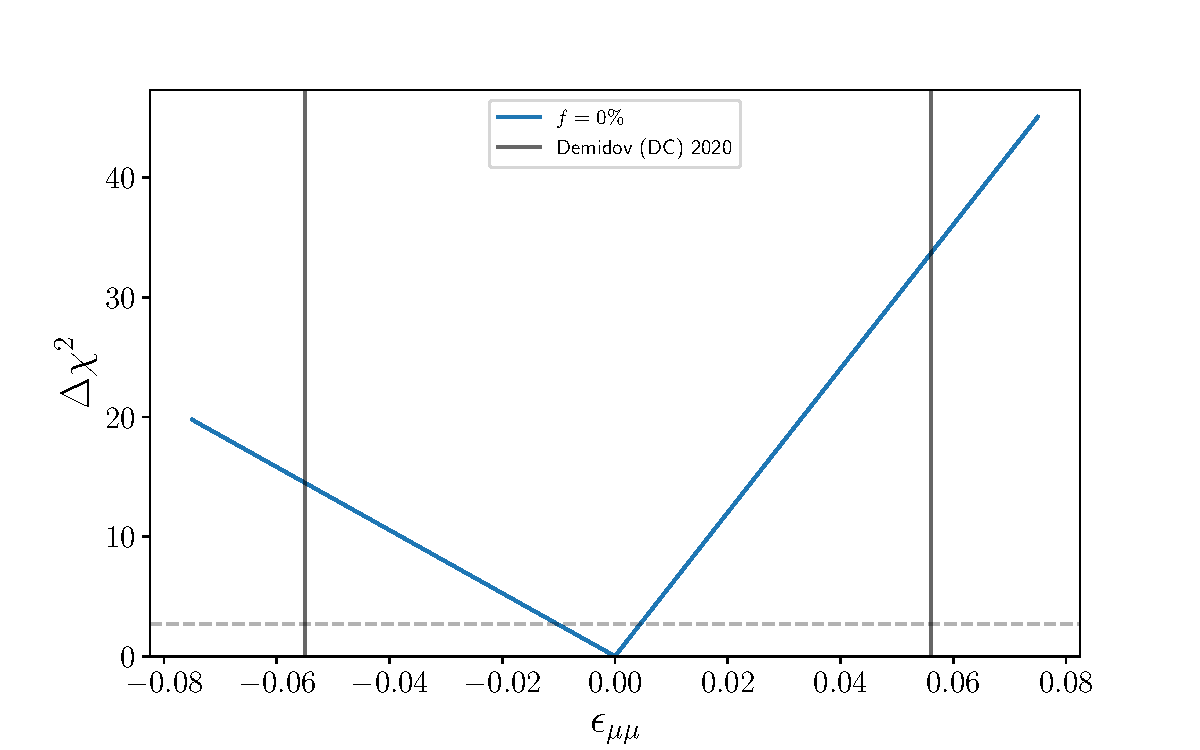
\includegraphics[width=0.4\linewidth]{figures/PINGU_emm.pdf}
       %\includegraphics[width=0.4\linewidth]{figures/PINGU_emt.pdf}
    \end{center}
    \caption{Expected pulls of predicted event numbers for PINGU. We compare the NSI event count with $\emt=-0.05$
    to the standard interaction count}\label{fig:PINGU_chisq}
 \end{figure}

 \begin{figure}[!tb]
    \begin{center}
       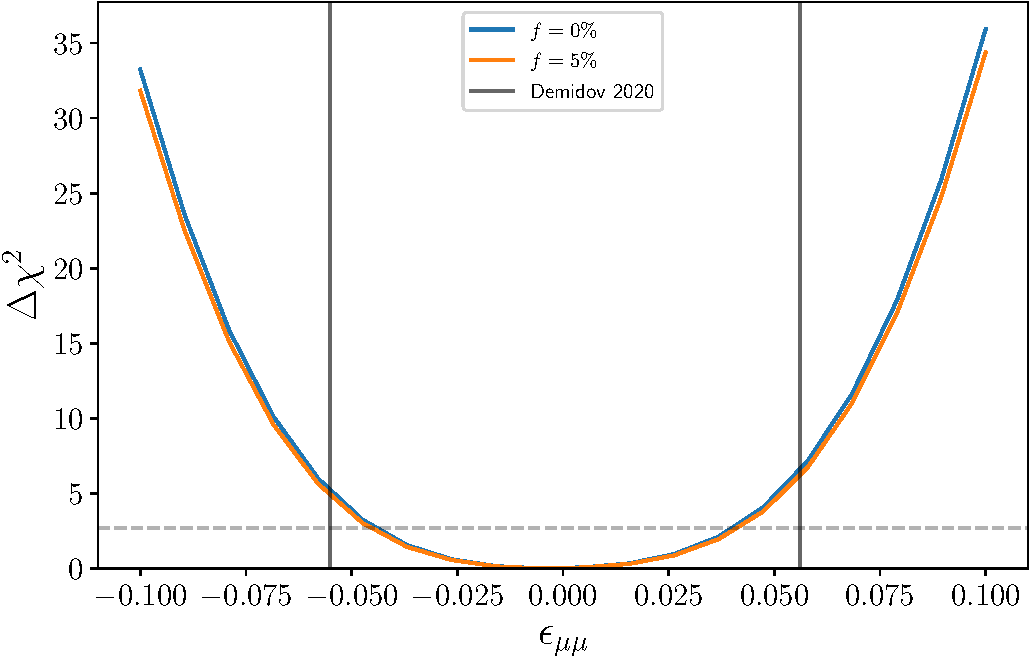
\includegraphics[width=0.4\linewidth]{figures/DC_emm.pdf}
       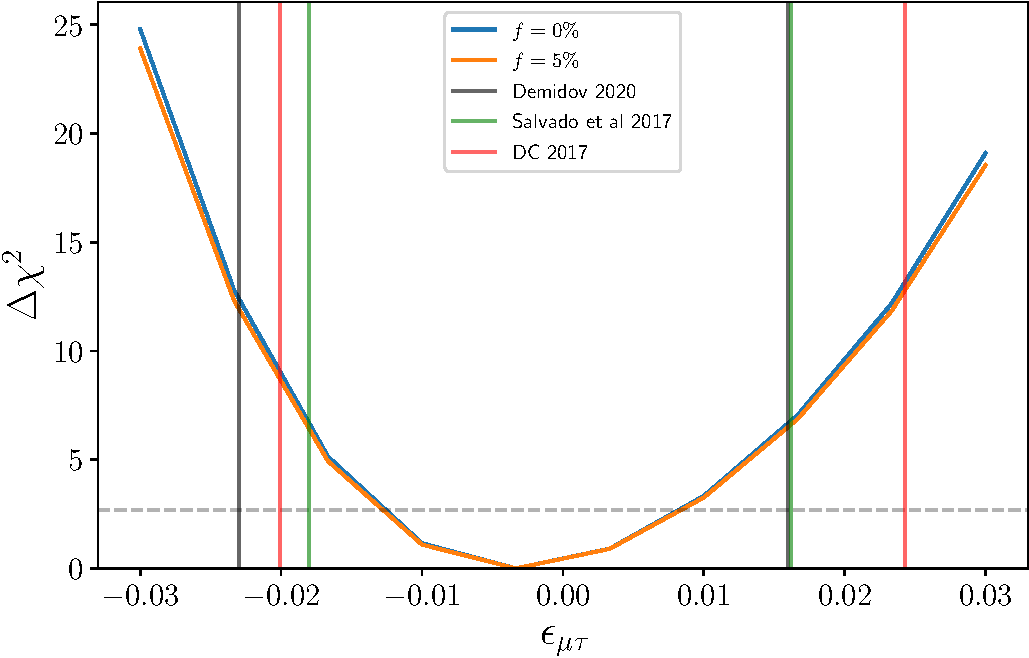
\includegraphics[width=0.4\linewidth]{figures/DC_emt.pdf}
    \end{center}
    \caption{Confidence levels from this analysis on the NSI
    parameters for systematic error and without. The black lines show the 90\% credibility region from~\cite{demidov}.}\label{fig:DC_chisq}
 \end{figure}

For the joint analysis, we follow the parameter goodness-of-fit prescription~\cite{maltoni2003} and construct the joint $\chi^2$ as 
\begin{align}
    \chi^2_{joint} = \chi^2_{IC} + \chi^2_{DC} + \chi^2_{P} - \chi^2_{IC,min} - \chi^2_{DC,min} - \chi^2_{P,min}\,
\end{align}
with test statistic $\chi^2_{joint,min}$.

\begin{figure}[!tb]
    \begin{center}
       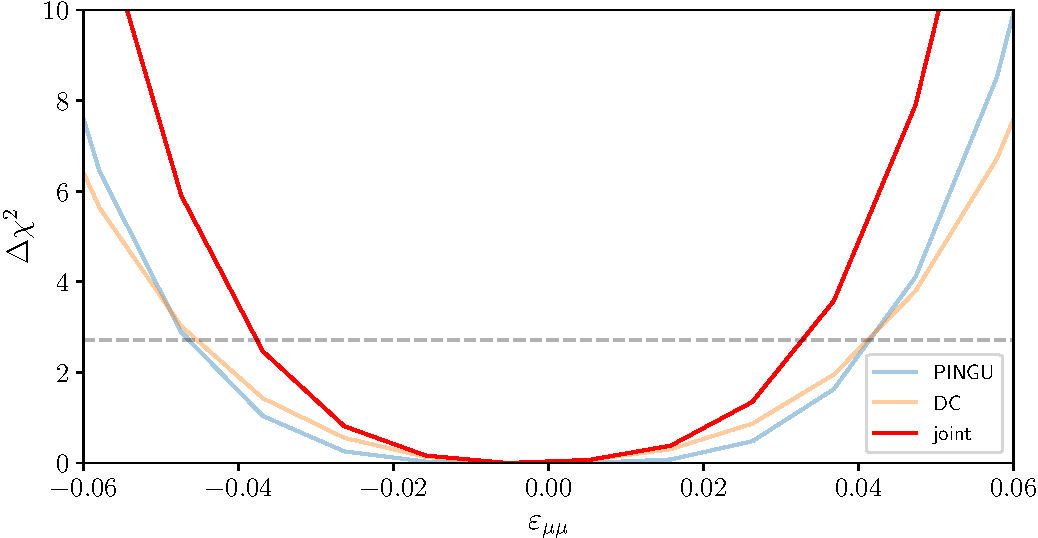
\includegraphics[width=0.4\linewidth]{figures/emm_deltachi.pdf}
    \end{center}
    \caption{}\label{fig:emm_deltachi}
 \end{figure}

 \begin{figure}[!tb]
    \begin{center}
       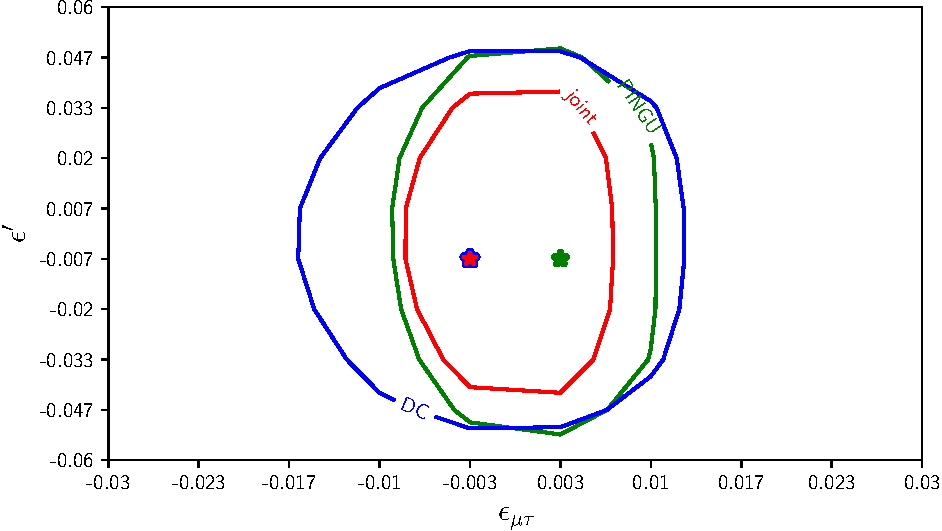
\includegraphics[width=0.4\linewidth]{figures/emm_emp_contour.pdf}
    \end{center}
    \caption{}\label{fig:emm_emp_contour}
 \end{figure}
At $90\%$ CL:
PINGU: $-0.046 < \emm < 0.041$
DC: $-0.045 < \emm < 0.041$
joint: $-0.038 < \emm < 0.033$
\begin{figure}[!tb]
    \begin{center}
       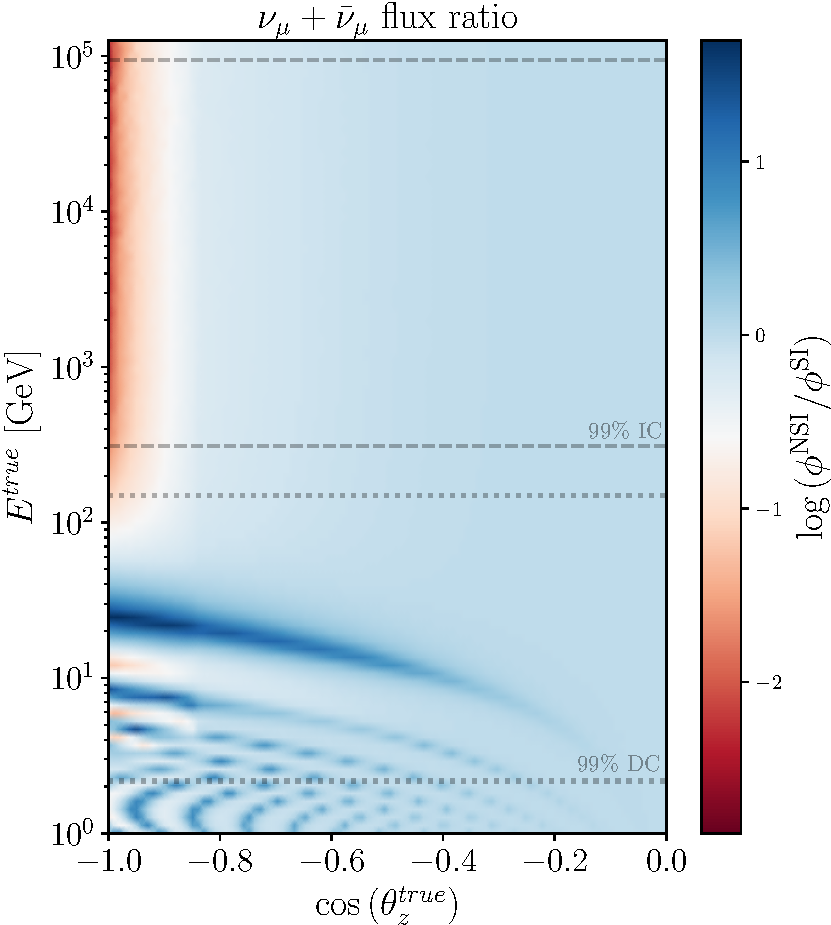
\includegraphics[width=0.4\linewidth]{figures/track_flux_ratio.pdf}
       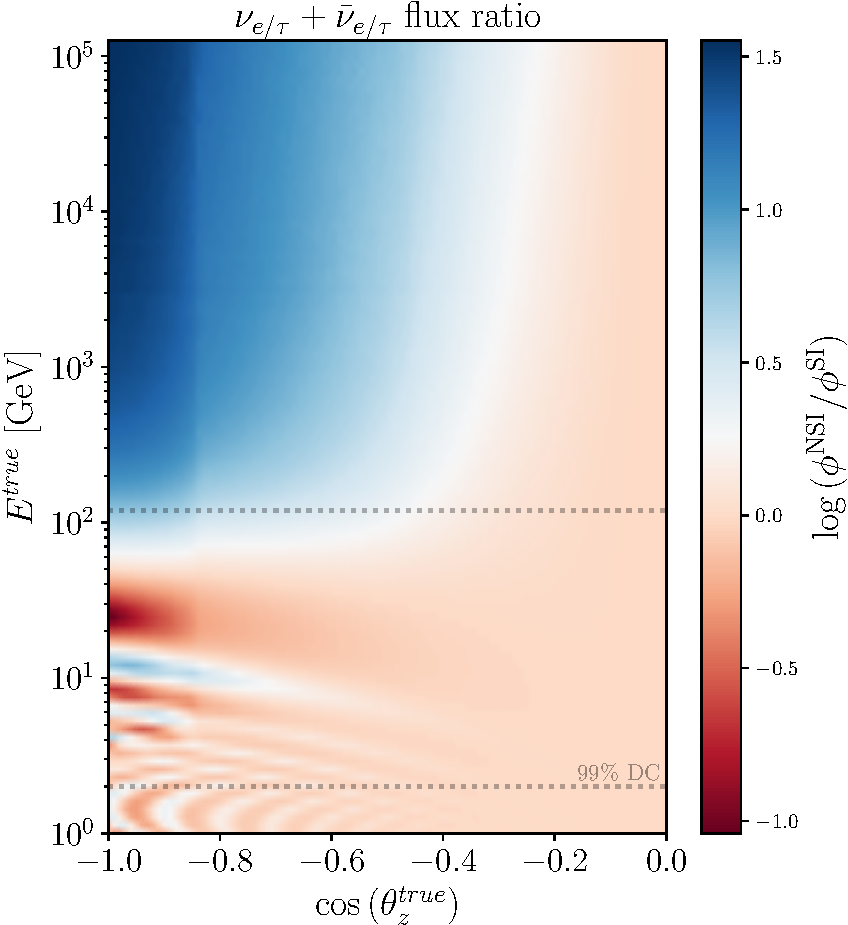
\includegraphics[width=0.4\linewidth]{figures/cascade_flux_ratio.pdf}
    \end{center}
    \caption{Ratio of NSI to SI atmospheric fluxes at detector level. Dotted (dashed) lines show the region in which 99\% of the 
    DeepCore (IceCube) MC events are contained.}\label{fig:flux_ratio}
 \end{figure}
\bibliographystyle{elsarticle-num}
\bibliography{article}
\end{document}


